\documentclass[a4paper, 14pt]{extarticle}

% Поля
%--------------------------------------
\usepackage{geometry}
\geometry{a4paper,tmargin=2cm,bmargin=2cm,lmargin=3cm,rmargin=1cm}
%--------------------------------------


%Russian-specific packages
%--------------------------------------
\usepackage[T2A]{fontenc}
\usepackage[utf8]{inputenc} 
\usepackage[english, main=russian]{babel}
%--------------------------------------

\usepackage{textcomp}

% Красная строка
%--------------------------------------
\usepackage{indentfirst}               
%--------------------------------------             


%Graphics
%--------------------------------------
\usepackage{graphicx}
\graphicspath{ {./images/} }
\usepackage{wrapfig}
%--------------------------------------

% Полуторный интервал
%--------------------------------------
\linespread{1.3}                    
%--------------------------------------

%Выравнивание и переносы
%--------------------------------------
% Избавляемся от переполнений
\sloppy
% Запрещаем разрыв страницы после первой строки абзаца
\clubpenalty=10000
% Запрещаем разрыв страницы после последней строки абзаца
\widowpenalty=10000
%--------------------------------------

%Списки
\usepackage{enumitem}

%Подписи
\usepackage{caption} 

%Гиперссылки
\usepackage{hyperref}

\hypersetup {
	unicode=true
}

%Рисунки
%--------------------------------------
\DeclareCaptionLabelSeparator*{emdash}{~--- }
\captionsetup[figure]{labelsep=emdash,font=onehalfspacing,position=bottom}
%--------------------------------------

\usepackage{tempora}

%Листинги
%--------------------------------------
\usepackage{listings}
\lstset{
	basicstyle=\ttfamily\footnotesize, 
	%basicstyle=\footnotesize\AnkaCoder,        % the size of the fonts that are used for the code
	breakatwhitespace=false,         % sets if automatic breaks shoulbd only happen at whitespace
	breaklines=true,                 % sets automatic line breaking
	captionpos=t,                    % sets the caption-position to bottom
	inputencoding=utf8,
	frame=single,                    % adds a frame around the code
	keepspaces=true,                 % keeps spaces in text, useful for keeping indentation of code (possibly needs columns=flexible)
	keywordstyle=\bf,       % keyword style
	numbers=left,                    % where to put the line-numbers; possible values are (none, left, right)
	numbersep=5pt,                   % how far the line-numbers are from the code
	xleftmargin=25pt,
	xrightmargin=25pt,
	showspaces=false,                % show spaces everywhere adding particular underscores; it overrides 'showstringspaces'
	showstringspaces=false,          % underline spaces within strings only
	showtabs=false,                  % show tabs within strings adding particular underscores
	stepnumber=1,                    % the step between two line-numbers. If it's 1, each line will be numbered
	tabsize=2,                       % sets default tabsize to 8 spaces
	title=\lstname                   % show the filename of files included with \lstinputlisting; also try caption instead of title
}
%--------------------------------------

%%% Математические пакеты %%%
%--------------------------------------
\usepackage{amsthm,amsfonts,amsmath,amssymb,amscd}  % Математические дополнения от AMS
\usepackage{mathtools}                              % Добавляет окружение multlined
\usepackage[perpage]{footmisc}
%--------------------------------------

%--------------------------------------
%			НАЧАЛО ДОКУМЕНТА
%--------------------------------------

\begin{document}
	
	%--------------------------------------
	%			ТИТУЛЬНЫЙ ЛИСТ
	%--------------------------------------
	\begin{titlepage}
		\thispagestyle{empty}
		\newpage
		
		
		%Шапка титульного листа
		%--------------------------------------
		\vspace*{-60pt}
		\hspace{-65pt}
		\begin{minipage}{0.3\textwidth}
			\hspace*{-20pt}\centering
			
\includegraphics[width=\textwidth]{emblem}
		\end{minipage}
		\begin{minipage}{0.67\textwidth}\small \textbf{
				\vspace*{-0.7ex}
				\hspace*{-6pt}\centerline{Министерство науки и высшего образования Российской Федерации}
				\vspace*{-0.7ex}
				\centerline{Федеральное государственное бюджетное образовательное учреждение }
				\vspace*{-0.7ex}
				\centerline{высшего образования}
				\vspace*{-0.7ex}
				\centerline{<<Московский государственный технический университет}
				\vspace*{-0.7ex}
				\centerline{имени Н.Э. Баумана}
				\vspace*{-0.7ex}
				\centerline{(национальный исследовательский университет)>>}
				\vspace*{-0.7ex}
				\centerline{(МГТУ им. Н.Э. Баумана)}}
		\end{minipage}
		%--------------------------------------
		
		%Полосы
		%--------------------------------------
		\vspace{-25pt}
		\hspace{-35pt}\rule{\textwidth}{2.3pt}
		
		\vspace*{-20.3pt}
		\hspace{-35pt}\rule{\textwidth}{0.4pt}
		%--------------------------------------
		
		\vspace{1.5ex}
		\hspace{-35pt} \noindent \small ФАКУЛЬТЕТ\hspace{80pt} <<Информатика и системы управления>>
		
		\vspace*{-16pt}
		\hspace{47pt}\rule{0.83\textwidth}{0.4pt}
		
		\vspace{0.5ex}
		\hspace{-35pt} \noindent \small КАФЕДРА\hspace{50pt} <<Теоретическая информатика и компьютерные технологии>>
		
		\vspace*{-16pt}
		\hspace{30pt}\rule{0.866\textwidth}{0.4pt}
		
		\vspace{11em}
		
		\begin{center}
			\Large {\bf Лабораторная работа №3} \\ 
			\large {\bf по курсу <<Языки и методы программирования>>} \\
			\large <<Полиморфизм на основе интерфейсов в языке Java>> 
		\end{center}\normalsize
		
		\vspace{8em}
		
		
		\begin{flushright}
			{Студент группы ИУ9-22Б Тараканов В. Д. \hspace*{15pt}\\ 
				\vspace{2ex}
				Преподаватель Посевин Д. П.\hspace*{15pt}}
		\end{flushright}
		
		\bigskip
		
		\vfill
		
		
		\begin{center}
			\textsl{Москва 2024}
		\end{center}
	\end{titlepage}
	%--------------------------------------
	%		КОНЕЦ ТИТУЛЬНОГО ЛИСТА
	%--------------------------------------
	
	\renewcommand{\ttdefault}{pcr}
	
	\setlength{\tabcolsep}{3pt}
	\newpage
	\setcounter{page}{2}
	
	\section{Задание}\label{Sect::task}
	
Класс квадратных целочисленных матриц размера n с порядком на основе количества
элементов, нарушающих симметричность матрицы относительно главной диагонали.
	
	\section{Результаты}\label{Sect::res}
	

	\begin{figure}[!htb]
		\begin{lstlisting}[language={},caption={Класс SquareMatrix, в котором реализована программа по заданию},label={lst:code1}]
		public class SquareMatrix implements Comparable<SquareMatrix>{
			private int[][] matrix;
			private  int n;
			public SquareMatrix(int n, int[][] matrix){
				this.matrix = matrix;
				this.n = n;
			}
			public int takeElem(int i, int j, int[][] matrix){
				return matrix[i][j];
			}
			public String toString(){
				String mat = "";
				for(int i = 0;i<this.n;i++){
					for(int j = 0;j<this.n;j++){
						mat+=this.matrix[i][j]+" ";
					}
					mat+="\n";
				}
				return mat;
			}
			public int countofElems(int[][] matrix){
				int cnt = 0;
				for(int i = 0;i<this.n-1;i++){
					for(int j = i+1;j<this.n;j++){
						if (takeElem(i,j,matrix)!=takeElem(j,i,matrix)){
							cnt++;
						}
					}
				}
				return cnt;
			}
			public int compareTo(SquareMatrix obj){
				return countofElems(this.matrix)-countofElems(obj.matrix);
			}
		}
		
			
		\end{lstlisting}
	\end{figure}
	
	\newpage
	
	\begin{figure}[!htb]
		\begin{lstlisting}[language={},caption={Класс Main, в котором реализована проверка работы класса SquareMatrix},label={lst:code2}]
			import java.util.Arrays;
			
			public class Main {
				public static void main(String[] args) {
					int[][] arr1 = {{1,1,2},{50,1,200},{100,1,1}};
					int[][] arr2 = {{1,1,2},{1,1,2},{1,1,1}};
					int[][] arr3 = {{1,1,2},{1,1,3},{2,3,1}};
					SquareMatrix[] a = new SquareMatrix[] {
						new SquareMatrix(3,  arr1),
						new SquareMatrix(3,arr2),
						new SquareMatrix(3, arr3)
					};
					Arrays.sort(a);
					for (SquareMatrix s: a){
						System.out.println(s);
					}
				}
				
			}
		\end{lstlisting}
	\end{figure}
	
	Результат запуска представлен на рисунке~\ref{fig:img1}.
	
	\begin{figure}[!htb]
		\centering
		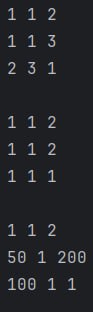
\includegraphics[width=0.2\textwidth]{img1}
		\caption{Результат}
		\label{fig:img1}
	\end{figure}
	
\end{document}
